\documentclass[aps, pra, amsfonts, a4paper, showpacs]{revtex4-1}
\usepackage{graphicx,graphics,epsfig}   
\usepackage{dcolumn}    
\usepackage{bm}         
\usepackage{subfigure}  
\usepackage{times,natbib}
\usepackage{amsmath,amsfonts,amssymb,graphics,graphicx,epsfig,color,times,natbib}
\usepackage{xcolor}
\usepackage{braket}
\usepackage{amsmath}
\usepackage{bbold}

\newcommand{\todo}[1]{\textcolor{red}{\texttt{TODO: #1}}}


\begin{document}

\newcommand{\kpz}{\ket{\psi_0}}
\newcommand{\bpz}{\bra{\psi_0}}
\newcommand{\hz}{\braket{H_0}}
\newcommand{\hsqz}{\braket{H^2_0}}

\section*{Estimate of Zeno time for hyperfine flip-flops}

Say we start out in a state $\ket{\psi_0}=\ket{\uparrow}\otimes\ket{\phi_0}$, where $\ket{\phi_0}$ is some nuclear state. This is approximately the case after many consecutive cross-polarized detections, which tell us that the nuclear state $\ket{\phi_0}$ is most probably the nuclear state that puts the transition on resonance. 

What is the timescale at which we could Zeno-inhibit the hyperfine evolution (``decay'') of this state? 

\vspace{0.5cm}
Let's start out with the standard expression for the Zeno time $\tau_Z$ \cite{pascazio_all_2014}
\[
\bpz e^{-i H t} \kpz = 1 - i\hz t -\frac{1}{2} \hsqz t^2
\]
where $ \hsqz = \bpz | H^2 | \kpz$ and similar for $\hz$.
Then the probability to find the system in state $\kpz$ after a short time $t$ is given by
\begin{equation}
p_0(t) \approx 1- (\hsqz - \hz^2)t^2 \equiv 1- \frac{t^2}{\tau_z^2} 
\label{Eq: p0}
\end{equation}
for $t \ll \tau_Z$.

The full spin Hamiltonian for an external magnetic field along $\hat{z}$ is
\begin{equation}
H=\Omega S^z + \sum_k \omega_k I^z_k + \sum_k A_k I^z_k S^z + \sum_k \frac{A_k}{2}(S^zI^-_k + S^- I_k^+)
\label{Eq: H}
\end{equation}
where the index $k$ runs over all nuclear sites. Denoting the flip-flop term
\[H_{int} = \sum_k \frac{A_k}{2}(S^zI^-_k + S^- I_k^+) \]
and assuming that $\kpz$ be an eigenstate of $H-H_{int}$ one obtains
\begin{equation}
\frac{1}{\tau_z^2} = \sum_n |\braket{\psi_0|H_{int}|\psi_n}|^2
\label{Eq: simp}
\end{equation}
where $\{\ket{\psi_n}\}$ is an orthonormal basis of the electron-nuclear spin system, while $\{\ket{\phi_n}\}$ is a basis of the nuclear system alone.
Assuming the form $\ket{\psi_0}=\ket{\uparrow}\otimes\ket{\phi_0}$ for the initial state, the above expression for $\tau_Z$ simplifies to
\begin{equation}
\begin{split}
\frac{1}{\tau_z^2} &=\sum_n |\braket{\phi_0 | \sum_k \frac{A_k}{2} I_k^+ |\phi_n}|^2 \\
&= \sum_k \sum_l \frac{A_k A_l}{4}\braket{\phi_0 | I_k^+ I_l^- |\phi_0} \\
&= \sum_k \frac{A_k^2}{4}(J_k(J_k+1) - m_k(m_k -1)).
\end{split}
\end{equation}
Here the numbers $m_k$ ($J_k$) denote the z-component (maximum projection) of the $k$th spin in the initial nuclear state $\ket{\phi_0}$.

Let's talk about two questions:
\begin{itemize}
\item Can we measure fast enough for a realistic distribution $\{A_k\}$?
\item How do we tell if we observe this Zeno effect or not?
\end{itemize}

We address the first question by computing values of $\tau_Z$ for a range of coupling strength distributions $\{ A_k \}$. Taking $\hat{z}$ along the growth axis of the quantum dot, we assume that the wavefunction follows a Gaussian distribution with a cutoff in the $x-y$ plane and is constant along $\hat{z}$. There are three parameters to describe such a distribution: the radius in the $x-y$ plane beyond which we set the coupling to zero is denoted $r$. The number of atomic layers in the $\hat{z}$ direction is $N_z$ and the decay constant is denoted $R$. Hence
\begin{equation}
A_{(x,y)}=\frac{A_{tot}}{N_z}\frac{\exp(-\alpha(x^2+y^2))m_{(x,y)}}{\sum_{(x,y)}\exp(-\alpha(x^2+y^2))m_{(x,y)}}
\label{Eq: dist}
\end{equation}
where
\[\begin{split}
m_{(x,y)}&= 1\ \  \mathrm{for}\ x^2+y^2<r^2 \\
 &= 0\ \  \mathrm{else}
\end{split}\] and where the indices $x,y$ take on integer values.
We assume nuclear spin $J_k=\frac{1}{2}$ and a nuclear spate in which the flipable spins are uniformly distributed. Furthermore take $N_z=10$.
The plots presented in Fig. \ref{Fig: tz} show that Zeno times seem to lie in the nanosecond regime under these assumptions.

\begin{figure}
    \centering
    \begin{minipage}{.5\textwidth}
        \centering
        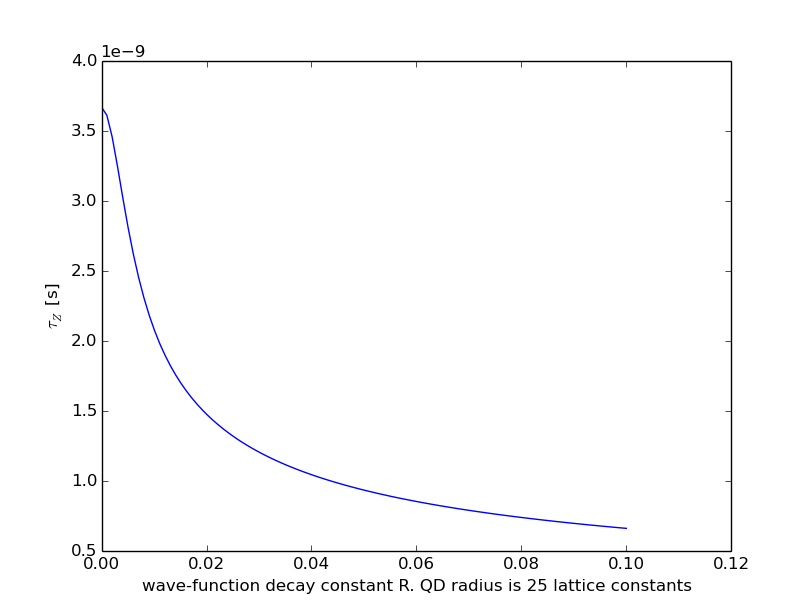
\includegraphics[width=\linewidth]{tz_vs_R.png}
        \caption{Zeno time vs. decay constant $R$ at a radius $r=25$.}
    \end{minipage}%
    \begin{minipage}{0.5\textwidth}
        \centering
        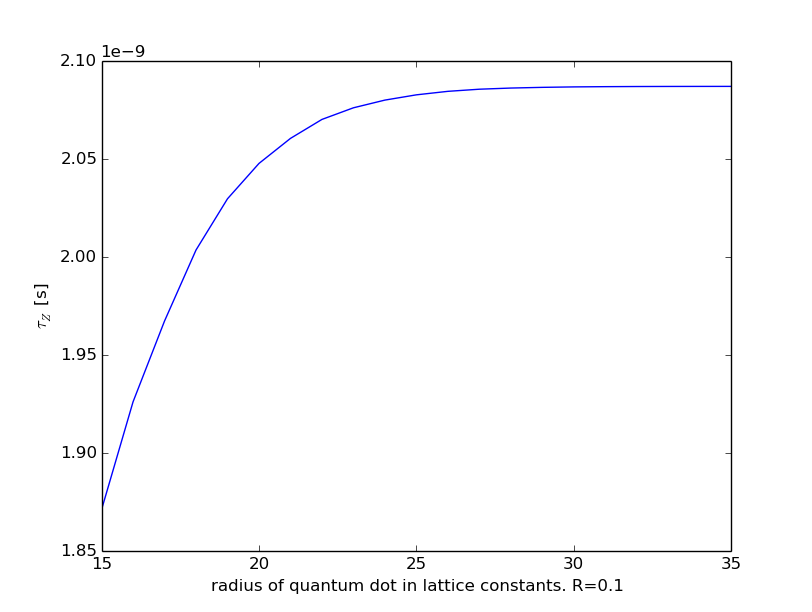
\includegraphics[width=\linewidth]{tz_vs_radius.png}
        \caption{Zeno time vs. cutoff radius $r$ for decay constant $R=0.1$.}
    \end{minipage}
    \label{Fig: tz}
\end{figure}

\bibliography{Refs_zeno}
\end{document}